\section{Inverted Pendulum Control System}
\subsection{Inverted Pendulum System}
Consider an inverted pendulum as shown in \autoref{fig:IPS}. 
The system consists of a cart with mass $M$ and a pendulum with mass $m_1$ and length $l$. The angle of the pendulum with respect to the vertical axis 
is denoted by $\theta$, the cart position is $x$, and the control input 
(force applied to the cart) is $u$.
\begin{figure}[htbp]
	\centering
	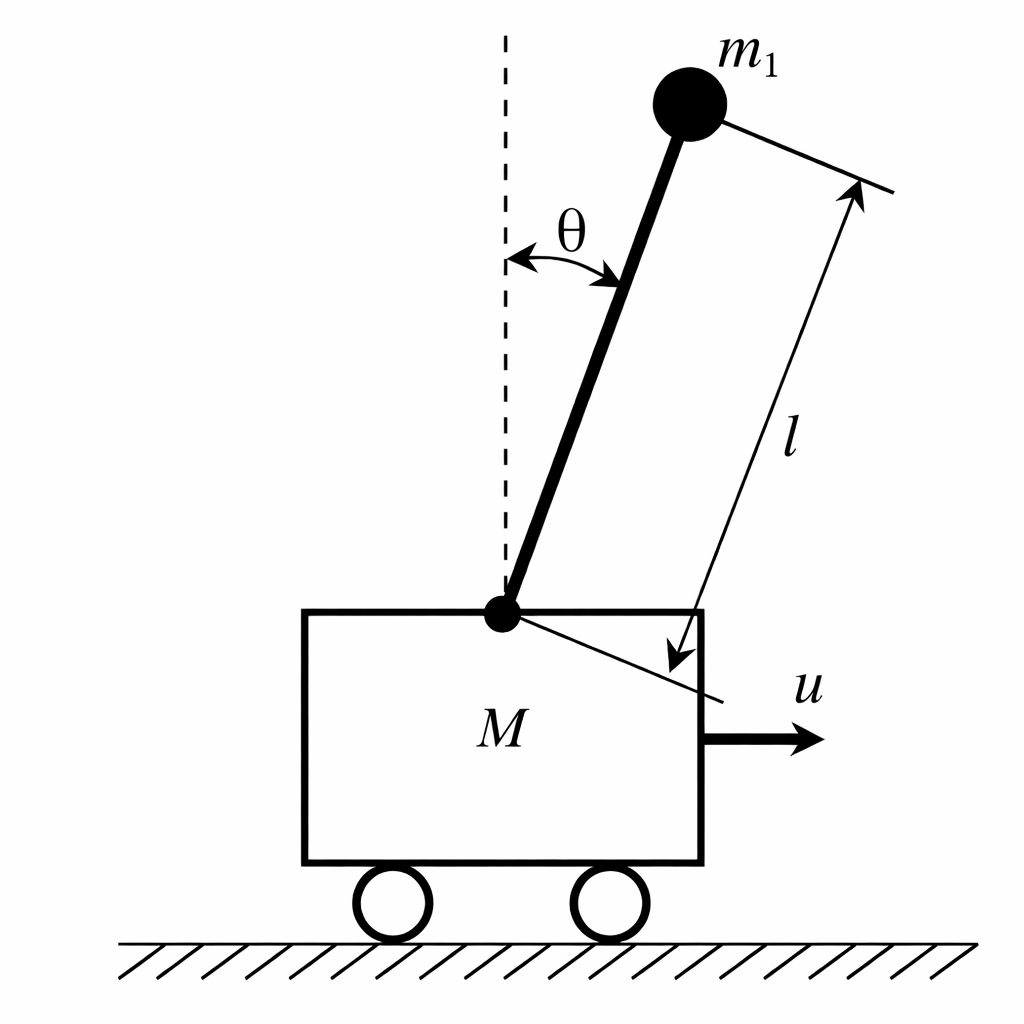
\includegraphics[width=0.45\linewidth]{images/IPS.png}
	\caption{Inverted Pendulum System}
	\label{fig:IPS}
\end{figure}

The nonlinear dynamic equations of the system and MATLAB code in Appendix I, are given by
\begin{equation}
	\ddot{\theta} =
	\frac{u \cos\theta - (M + m_1)g \sin\theta + m_1 l (\cos\theta \sin\theta) \dot{\theta}}
	{m_1 l (\cos\theta)^2 - (M + m_1)l}
\end{equation}
\begin{equation}
	\ddot{x} =
	\frac{u + m_1 l (\sin\theta) \dot{\theta}^2 - m_1 g \cos\theta \sin\theta}
	{M + m_1 - m_1 (\cos\theta)^2}
\end{equation}
where:
\begin{itemize}
	\item $M = 5\,\text{kg}$ is the cart mass,
	\item $m_1 = 0.5\,\text{kg}$ is the pendulum mass,
	\item $l = 2\,\text{m}$ is the pendulum length,
	\item $g = 9.80665\,\text{m/s}^2$ is the gravitational acceleration.
\end{itemize}

The initial conditions of the system are selected as:
$\theta(0) = 0, \dot{\theta}(0) = 0$.

The control problem is to design a controller that stabilizes the pendulum around $\theta = 0$ while ensuring that the cart position tracks the reference value \textcolor{red}{$x = 30 (SV1)$}.

\subsection{Fuzzy control system design}
The inverted pendulum system is controlled using fuzzy logic controller composed of 81 rules, as presented in \autoref{tab:full_rule_base}. The controller employs four input variables, namely the pendulum angle $\theta$, angular velocity $\Delta\theta$, cart position $x$, and cart velocity $\Delta x$. 
\[
\left\{
\begin{aligned}
	\theta &\in [-0.3,\,0.3] \, (\mathrm{rad}) 
	&\Rightarrow\; K_{1} &= \frac{1}{0.3} \\[6pt]
	\dot{\theta} &\in [-1,\,1] \, \left(\mathrm{rad/s}\right) 
	&\Rightarrow\; K_{2} &= 1 \\[6pt]
	x &\in [-3,\,3] \, (\mathrm{m}) 
	&\Rightarrow\; K_{3} &= \frac{1}{3} \\[6pt]
	\dot{x} &\in [-3,\,3] \, \left(\mathrm{m/s}\right) 
	&\Rightarrow\; K_{4} &= \frac{1}{3}
\end{aligned}
\right.
\]
As illustrated in \autoref{fig:IPS_simu}, the Simulink block diagram of the inverted pendulum balance control system based on fuzzy logic consists of the reference input, error computation, fuzzy inference controller, and the nonlinear inverted pendulum plant. The fuzzy controller processes the system states and generates the control force applied to the cart, ensuring that the pendulum remains balanced in the upright position while maintaining stable cart motion.
Each input variable is described by three linguistic terms: Negative (NE), Zero (ZE), and Positive (PO). The output variable is the control force $u(t)$, which is defined using five linguistic terms: Negative Big (NB), Negative Medium (NM), Zero (ZE), Positive Medium (PM), and Positive Big (PB). Since each input has three membership functions, the complete rule base consists of $3^4 = 81$ fuzzy rules.

\begin{figure}[t]
	\centering
	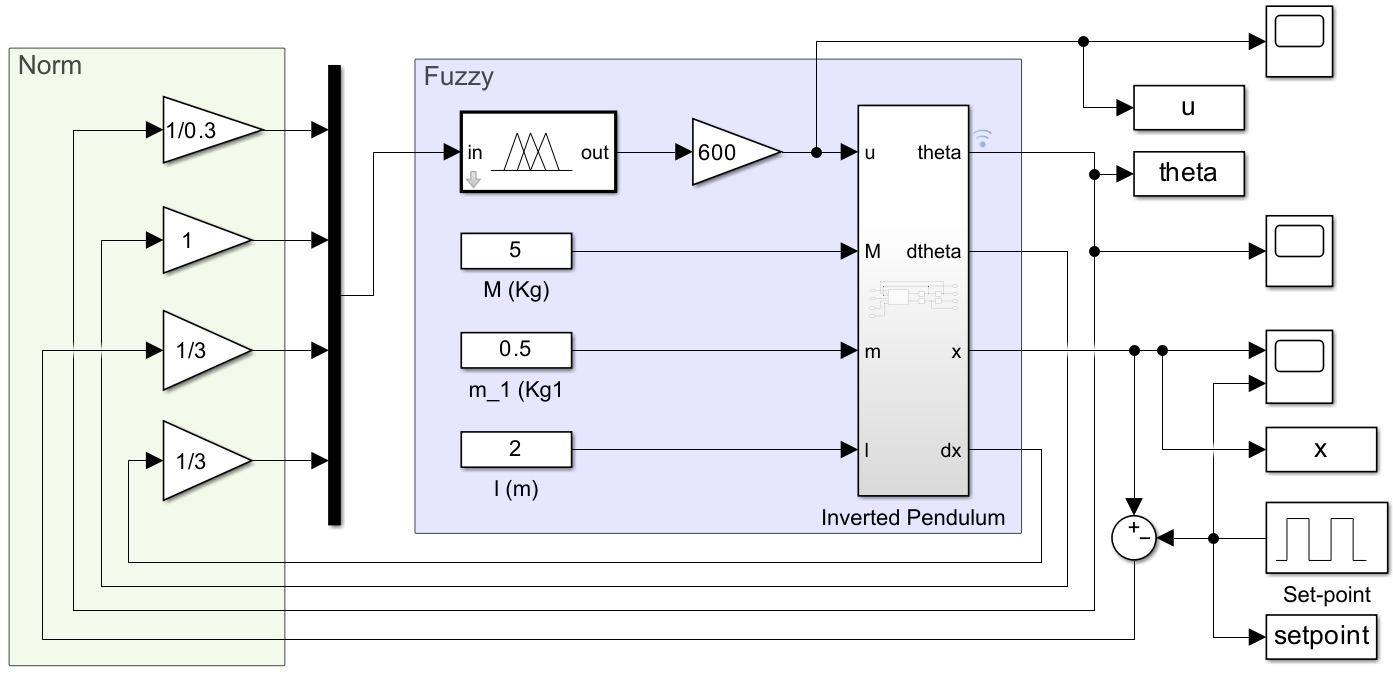
\includegraphics[width=\linewidth]{images/IPS_simulink.png}
	\caption{Simulink block diagram of the inverted pendulum balance control system using fuzzy logic.}
	\label{fig:IPS_simu}
\end{figure}

\begin{table*}[ht]
	\centering
	\caption{Fuzzy Rule Base for the Inverted Pendulum Controller}
	\label{tab:full_rule_base}
	
	\begin{minipage}{0.48\textwidth}
		\centering
		\begin{tabular}{cccccc}
			\toprule
			No. & $\theta$ & $\Delta\theta$ & $x$ & $\Delta x$ & $u$ \\
			\midrule
			1  & NE & NE & NE & NE & NB \\
			2  & NE & NE & NE & ZE & NB \\
			3  & NE & NE & NE & PO & NM \\
			4  & NE & NE & ZE & NE & NB \\
			5  & NE & NE & ZE & ZE & NM \\
			6  & NE & NE & ZE & PO & ZE \\
			7  & NE & NE & PO & NE & NM \\
			8  & NE & NE & PO & ZE & ZE \\
			9  & NE & NE & PO & PO & ZE \\
			10 & NE & ZE & NE & NE & NB \\
			11 & NE & ZE & NE & ZE & NM \\
			12 & NE & ZE & NE & PO & NM \\
			13 & NE & ZE & ZE & NE & NM \\
			14 & NE & ZE & ZE & ZE & ZE \\
			15 & NE & ZE & ZE & PO & ZE \\
			16 & NE & ZE & PO & NE & ZE \\
			17 & NE & ZE & PO & ZE & ZE \\
			18 & NE & ZE & PO & PO & PO \\
			19 & NE & PO & NE & NE & NM \\
			20 & NE & PO & NE & ZE & NE \\
			21 & NE & PO & NE & PO & ZE \\
			22 & NE & PO & ZE & NE & NE \\
			23 & NE & PO & ZE & ZE & ZE \\
			24 & NE & PO & ZE & PO & PO \\
			25 & NE & PO & PO & NE & ZE \\
			26 & NE & PO & PO & ZE & PO \\
			27 & NE & PO & PO & PO & PM \\
			28 & ZE & NE & NE & NE & NB \\
			29 & ZE & NE & NE & ZE & NM \\
			30 & ZE & NE & NE & PO & NM \\
			31 & ZE & NE & ZE & NE & NM \\
			32 & ZE & NE & ZE & ZE & ZE \\
			33 & ZE & NE & ZE & PO & ZE \\
			34 & ZE & NE & PO & NE & ZE \\
			35 & ZE & NE & PO & ZE & ZE \\
			36 & ZE & NE & PO & PO & PO \\
			37 & ZE & ZE & NE & NE & NM \\
			38 & ZE & ZE & NE & ZE & ZE \\
			39 & ZE & ZE & NE & PO & ZE \\
			40 & ZE & ZE & ZE & NE & ZE \\
			41 & ZE & ZE & ZE & ZE & ZE \\
			\bottomrule
		\end{tabular}
	\end{minipage}
	\hfill
	\begin{minipage}{0.48\textwidth}
		\centering
		\begin{tabular}{cccccc}
			\toprule
			No. & $\theta$ & $\Delta\theta$ & $x$ & $\Delta x$ & $u$ \\
			\midrule
			42 & ZE & ZE & ZE & PO & PO \\
			43 & ZE & ZE & PO & NE & ZE \\
			44 & ZE & ZE & PO & ZE & PO \\
			45 & ZE & ZE & PO & PO & PO \\
			46 & ZE & PO & NE & NE & NE \\
			47 & ZE & PO & NE & ZE & ZE \\
			48 & ZE & PO & NE & PO & PO \\
			49 & ZE & PO & ZE & NE & ZE \\
			50 & ZE & PO & ZE & ZE & PO \\
			51 & ZE & PO & ZE & PO & PO \\
			52 & ZE & PO & PO & NE & PO \\
			53 & ZE & PO & PO & ZE & PO \\
			54 & ZE & PO & PO & PO & PO \\
			55 & PO & NE & NE & NE & NE \\
			56 & PO & NE & NE & ZE & ZE \\
			57 & PO & NE & NE & PO & PO \\
			58 & PO & NE & ZE & NE & ZE \\
			59 & PO & NE & ZE & ZE & ZE \\
			60 & PO & NE & ZE & PO & PO \\
			61 & PO & NE & PO & NE & PO \\
			62 & PO & NE & PO & ZE & PO \\
			63 & PO & NE & PO & PO & PO \\
			64 & PO & ZE & NE & NE & ZE \\
			65 & PO & ZE & NE & ZE & ZE \\
			66 & PO & ZE & NE & PO & PO \\
			67 & PO & ZE & ZE & NE & ZE \\
			68 & PO & ZE & ZE & ZE & PO \\
			69 & PO & ZE & ZE & PO & PO \\
			70 & PO & ZE & PO & NE & PO \\
			71 & PO & ZE & PO & ZE & PO \\
			72 & PO & ZE & PO & PO & PO \\
			73 & PO & PO & NE & NE & NE \\
			74 & PO & PO & NE & ZE & ZE \\
			75 & PO & PO & NE & PO & PO \\
			76 & PO & PO & ZE & NE & ZE \\
			77 & PO & PO & ZE & ZE & ZE \\
			78 & PO & PO & ZE & PO & PO \\
			79 & PO & PO & PO & NE & PO \\
			80 & PO & PO & PO & ZE & PO \\
			81 & PO & PO & PO & PO & PO \\
			\bottomrule
		\end{tabular}
	\end{minipage}
	
\end{table*}

\subsection{Simulation Results}
\autoref{fig:IPS_results} illustrates the fuzzy control performance of the inverted pendulum system, including the cart position $x(t)$, pendulum angle $\theta(t)$, and control input $u(t)$. 
The cart position $x(t)$ reaches a peak of approximately $0.35\,\text{m}$. The percentage overshoot is therefore estimated as
\[
\%OS_{x(t)} = \frac{0.35 - 0.30}{0.30} \times 100 \approx 16.7\%.
\]
The system settles around the desired position with negligible steady-state error before the reference change.
At $t \approx 10\,\text{s}$, the reference switches from $0.3\,\text{m}$ to $0\,\text{m}$. The cart position exhibits a small undershoot of approximately $-0.05\,\text{m}$ before converging smoothly to zero, indicating good tracking capability and acceptable transient performance.
For the pendulum angle response, the maximum deviation during the first transient is approximately $0.045\,\text{rad}$, while after the reference change it reaches about $-0.04\,\text{rad}$.
The control input $u(t)$ large control effort (approximately $\pm 20\,\text{N}$) is applied during the initial balancing phase and at the switching instant ($t \approx 10\,\text{s}$). After each transient, the control signal quickly attenuates toward zero, demonstrating stable regulation and efficient energy usage while ensuring accurate tracking of the reference position.
\begin{figure}[ht]
	\centering
	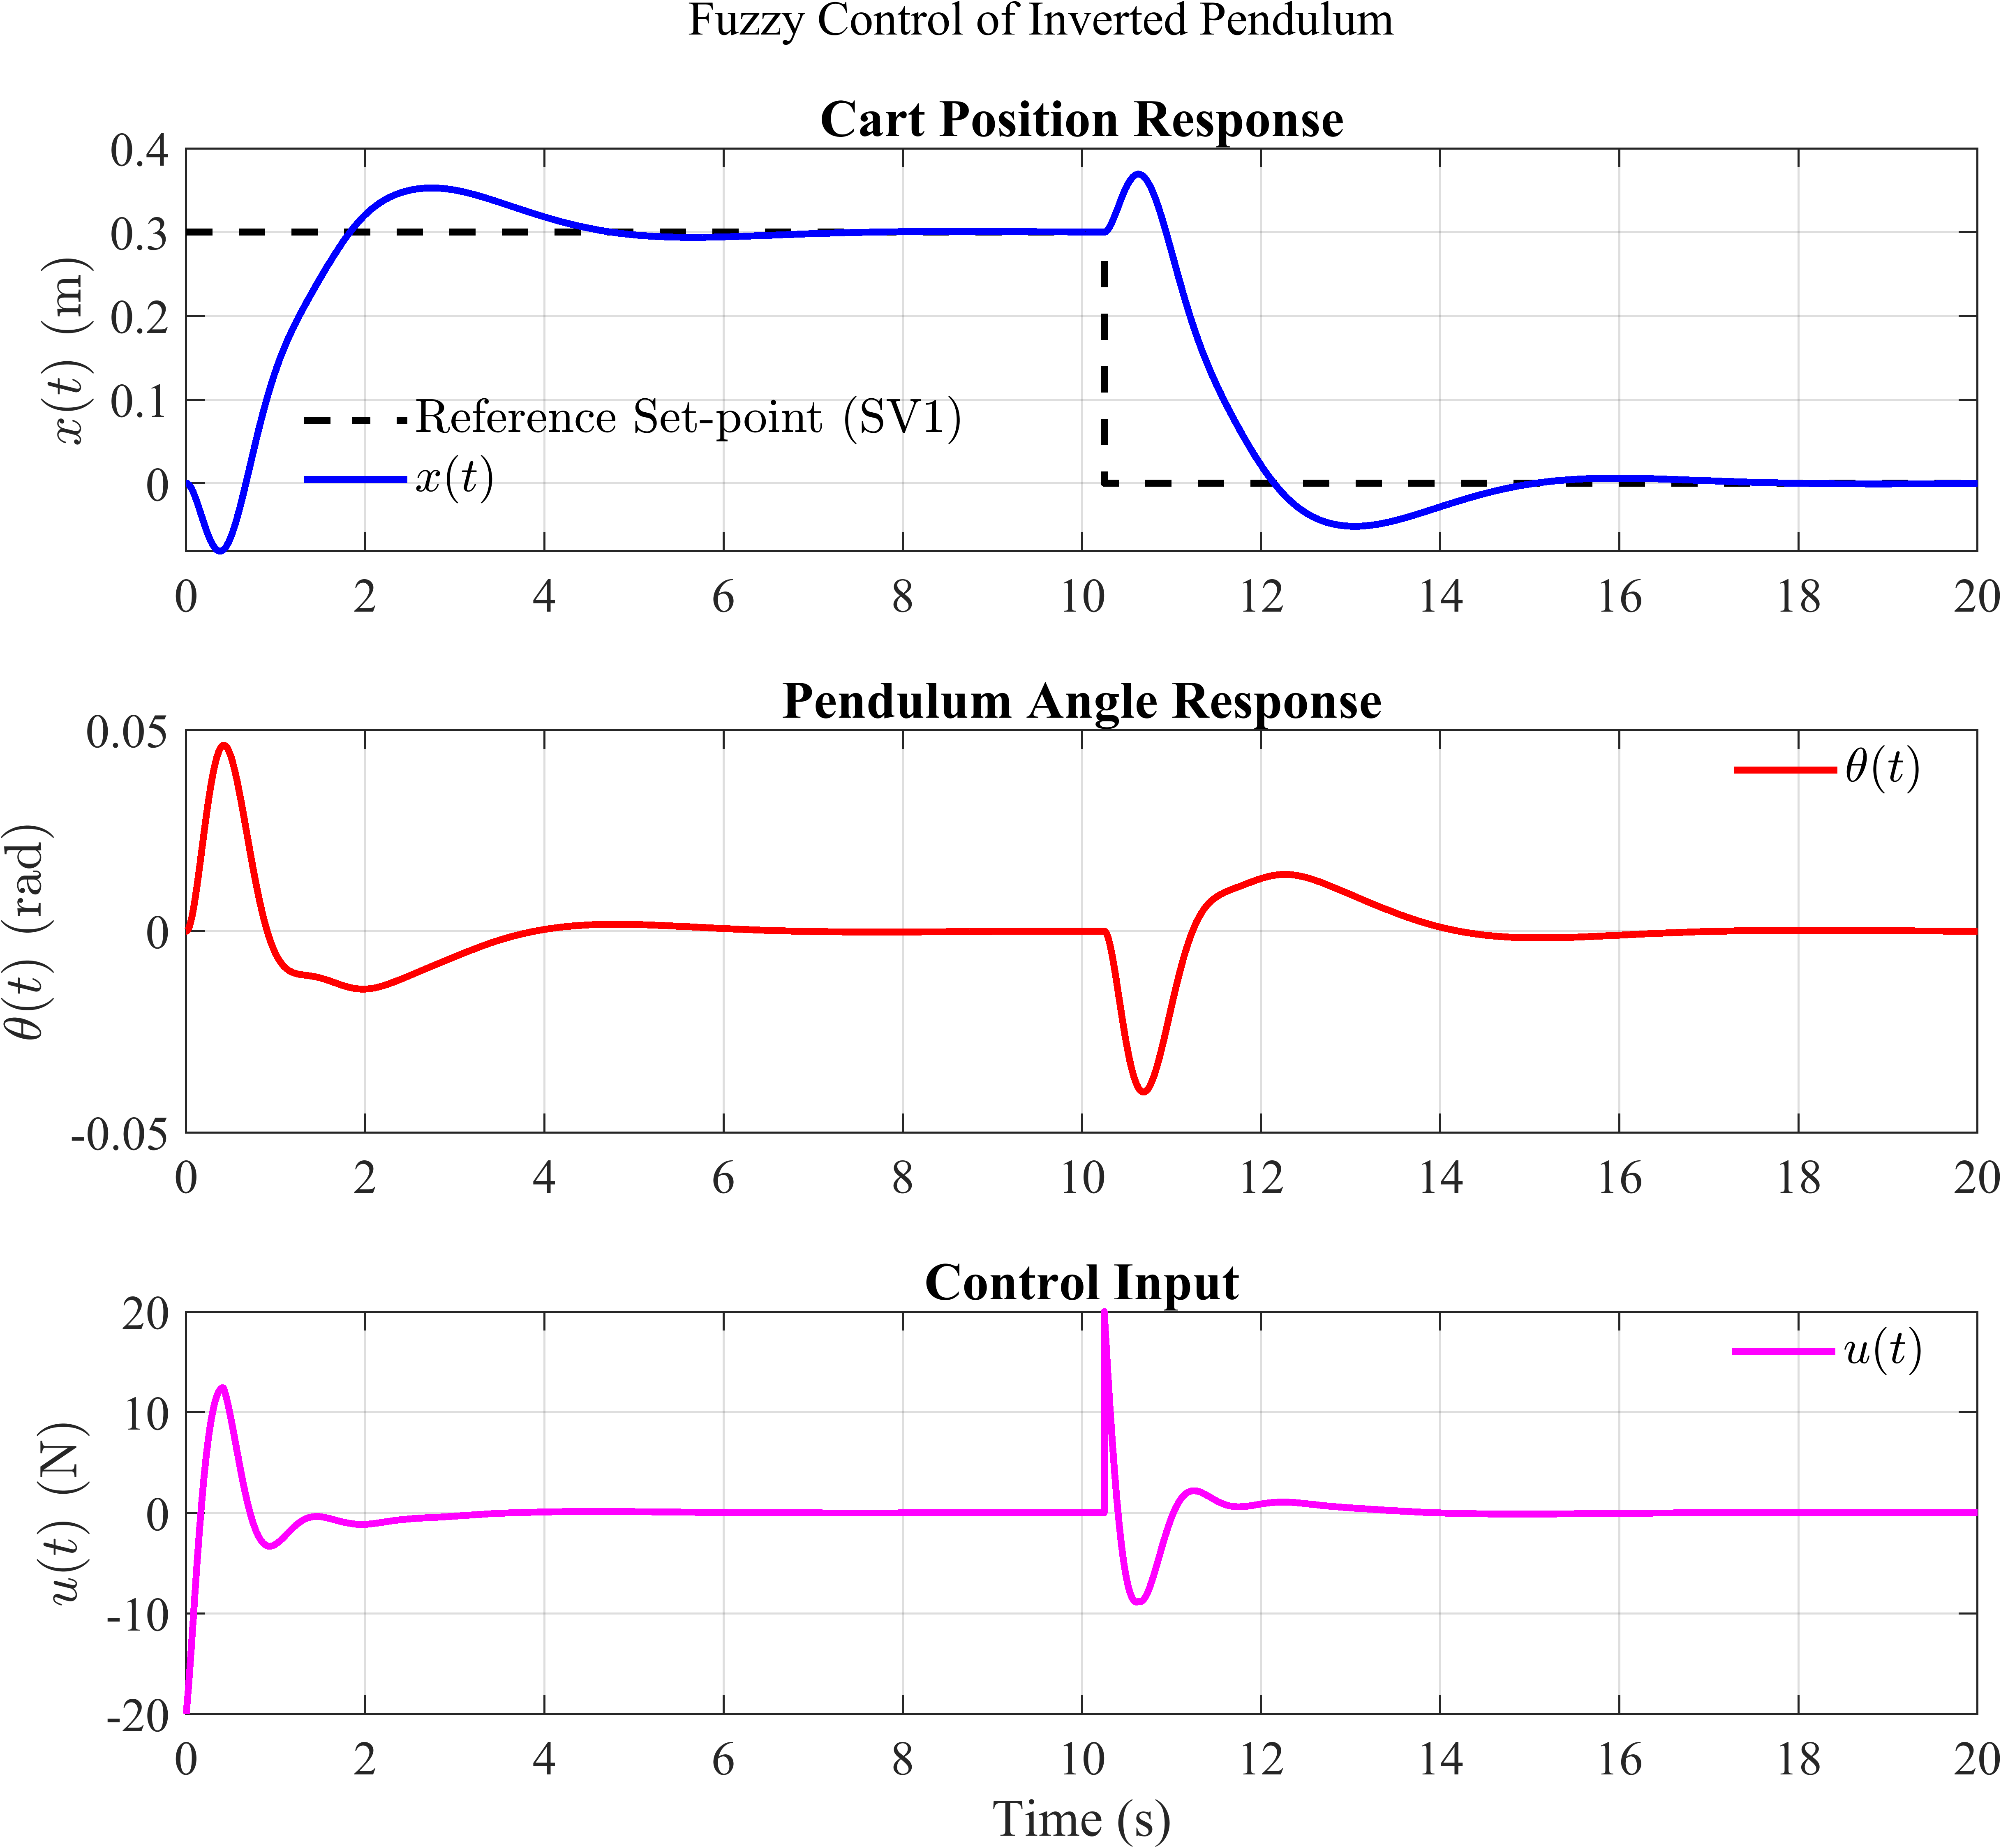
\includegraphics[width=\linewidth]{images/IPS_results.png}
	\caption{The Simulation Results of the Inverted Pendulum Balance Control System.}
	\label{fig:IPS_results}
\end{figure}